% ============================================================
%  hw3_statement.tex
%  Exact re-typesetting of hw3.pdf (MATH 6660, Homework 3, Fall 2026).
%  Statement only -- nothing added, nothing removed, nothing corrected.
%  Build:  pdflatex hw3_statement.tex
% ============================================================
%
%  Geometry measured from hw3.pdf:
%    paper 612 x 792 (letter);  text block x: 40.8 .. 551.0
%    header ink top y = 36.2 ; head rule y = 61.4 (full text width)
%    title ink top y = 81.7 ; folio ink top y = 723.0
%    section heading "Beam Equation": SFBX1440 (14.4pt bold), ink top y = 114.3,
%      NO underline rule (unlike HW1/HW2)
%    figure: 400x190 jpeg embedded in the original, ink spans
%      x 169.9..429.1 (259.2 wide), y 174.7..302.9
%    enumerate: label "1." at x = 54.0, item text at x = 67.9
%    fonts: cm-super T1 (SFRM1095 / SFBX1440 / SFCC1200 / SFTI1095)
%
\documentclass[11pt]{article}

\usepackage[letterpaper,left=40.9pt,right=61pt,top=77.2pt,bottom=90pt,
            headheight=30pt,headsep=15.6pt,footskip=28.3pt]{geometry}
\usepackage[T1]{fontenc}
\usepackage{amsmath,amssymb}
\usepackage{graphicx}
\usepackage{enumitem}
\usepackage{fancyhdr}
\usepackage{hyperref}

\pagestyle{fancy}
\fancyhf{}
\fancyhead[R]{\textbf{Assigned:} Monday Sept. 28, 2026\\
              \textbf{Due:} Monday Oct. 12, 2026}
\fancyfoot[C]{\thepage}
\renewcommand{\headrulewidth}{0.4pt}

\setlength{\parindent}{0pt}

% label "1." at x=54.0 (13.2pt in), item text at x=67.9 (27.1pt in)
\setlist[enumerate,1]{leftmargin=27.1pt,labelsep=5.5pt,
                      topsep=\hwtopsep,itemsep=9pt,parsep=0pt}

% section heading: bold, no rule
\newcommand{\hwsection}[1]{%
  \par\vspace{\hwsecA}%
  \noindent{\Large\bfseries #1}\par\nobreak
  \nointerlineskip\vspace{\hwsecC}%
}
\newcommand{\hwsecA}{-2.4pt}
\newcommand{\hwsecC}{3.2pt}
\newcommand{\hwtopsep}{9.1pt}
% colon separator: measured 3.06pt before, 10.8pt (=\quad) after -- a plain
% math \mathrel{:} would also put 3.06pt AFTER, which hw3.pdf does not have.
% After a display that ends an item, \item's \addvspace{\itemsep} is absorbed
% by \belowdisplayskip (addvspace keeps the max), so the only way to widen that
% gap is \belowdisplayskip itself.  Default at 11pt is 11pt; hw3.pdf shows
% 2.76pt / 4.48pt more after the two \[...\] displays.
\newlength{\bdsave}
\newcommand{\bdsk}[1]{\setlength{\belowdisplayskip}{#1}%
                      \setlength{\belowdisplayshortskip}{#1}}
\newcommand{\dispBiv}{15.38pt}
\newcommand{\dispBv}{15.38pt}
\newcommand{\cln}{\;{:}\quad}
\newcommand{\figA}{1.5pt}
\newcommand{\figB}{-4.4pt}

\begin{document}
\setlength{\bdsave}{\belowdisplayskip}

\begin{center}
  {\large\textsc{MATH 6660: Homework 3}}\\
  {\large\textsc{Fall 2026}}
\end{center}

\hwsection{Beam Equation}

Consider the Beam equation from mechanics with boundary conditions that model a
cantilever beam:
\vspace{0pt}
\begin{align*}
  \textbf{PDE} &\cln u^{(iv)} = f(x) \quad x\in(0,1)\,,\\
  \textbf{BC}  &\cln u(0)=0, \quad u'(0)=0, \quad u''(1)=0, \quad u'''(1)=0 .
\end{align*}

\par\vspace{\figA}
\noindent\makebox[\linewidth]{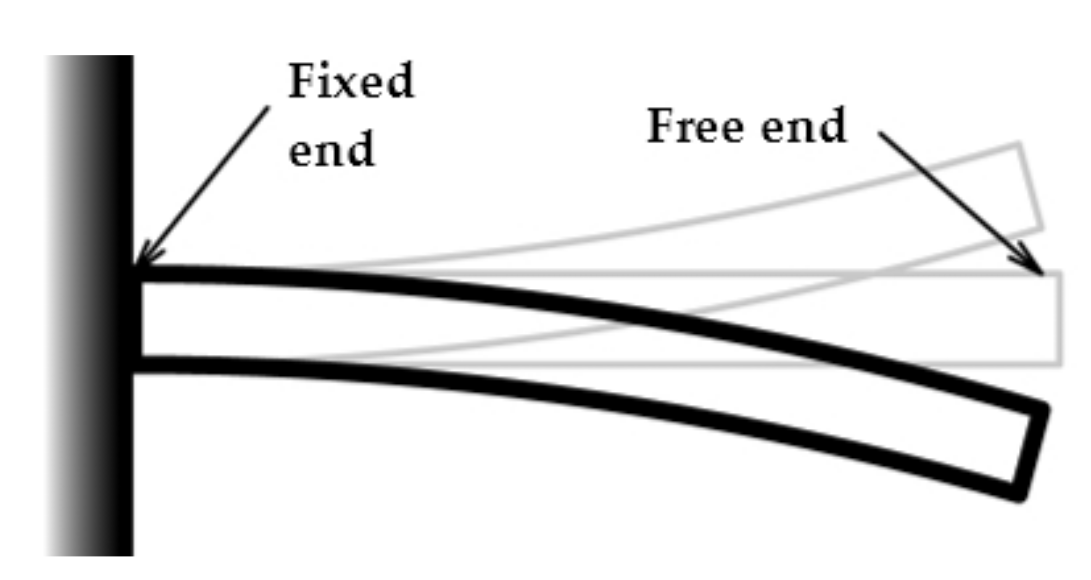
\includegraphics[width=209.5pt]{problem.png}}
\par\vspace{\figB}

\begin{enumerate}

\item Recast this problem as a variational problem. Clearly state the test and
trial function spaces.

\item Interpret the variational problem as an energy minimization problem,
clearly stating the energy functional. Prove that the variational problem and
the energy minimization problems are equivalent.

\item Develop a CG(3) finite element method for this problem.

\item Prove an \emph{a priori} error estimate for this method in the energy
norm:
\bdsk{\dispBiv}
\[
  \|e\|_{E} = \left\{\int_{0}^{1}\left(e''\right)^{2}\,dx\right\}^{1/2} .
\]

\item Prove an \emph{a priori} error estimate for this method in the $L_{2}$
norm:
\bdsk{\dispBv}
\[
  \|e\|_{L^{2}} = \left\{\int_{0}^{1}\left(e\right)^{2}\,dx\right\}^{1/2} .
\]

\item Numerically implement the cG(3) method on a uniform mesh with the
following functions
\bdsk{\bdsave}
\begin{align*}
  f(x) &= p_{1}(x)\cos(2\pi x) + p_{2}(x)\sin(2\pi x),\\
  p_{1}(x) &= -64\pi(18 - 6\pi^{4}x^{2} + 18x^{3}\pi^{2} + 2\pi^{4}x
              - 36\pi^{2}x^{2} - 27x + 12\pi^{2}x + 4\pi^{4}x^{3} + 3\pi^{2}),\\
  p_{2}(x) &= 216 - 816\pi^{2} - 96\pi^{4} + 32\pi^{6}x^{2} - 384\pi^{4}x^{3}
              - 64\pi^{6}x^{3} - 288\pi^{4}x^{2}\\
           &+ 3456\pi^{2}x + 576\pi^{4}x - 2592\pi^{2}x^{2}
              + 144\pi^{4}x^{4} + 32\pi^{6}x^{4},\\
  u(x) &= \bigl((18 + 2\pi^{2})x^{2} + (-24 - 4\pi^{2})x^{3}
           + (9 + 2\pi^{2})x^{4}\bigr)\sin(2\pi x).
\end{align*}
Numerically determine the convergence rate in both the energy norm and the
$L^{2}$-norm by creating an appropriate convergence table.

\end{enumerate}

\end{document}
